\documentclass[a4paper,DIV=17,dvipsnames,headsepline]{scrartcl}
\usepackage[utf8]{inputenc}
% \usepackage[margin=1in]{geometry}
\usepackage{graphicx}    % For including images
\usepackage{hyperref}    % For hyperlinks
\hypersetup{
    colorlinks=true,
    linkcolor=MidnightBlue,
    filecolor=magenta,      
    urlcolor=MidnightBlue,
    pdftitle={QuPath training},
    pdfpagemode=FullScreen,
    }
\usepackage{xcolor}      % For colored text (e.g., to highlight commands)
\usepackage{menukeys}   % forkeys and menu
\usepackage{listings}   % for code
\usepackage{siunitx}
\usepackage{lmodern}    % the font
\renewcommand{\familydefault}{\sfdefault}  % sans serif fonts
\usepackage{booktabs}   % nicer table
\usepackage{fourier}    % warning symbol
\pagestyle{headings}     % use srartcl headings style

\usepackage{enotez}      % create end notes with the solutions
\setenotez{backref=true}


\newcommand{\showsolutions}{\long\def\soln ##1\solnend{##1}}
\newcommand{\nosolutions}{\long\def\soln##1\solnend{}}

\showsolutions
%\nosolutions

\title{Nikon NIS-Elements\\ General Analysis 3}
\author{Dina Ratsimandresy, Jérôme Boulanger}
\date{May 2025}

\begin{document}

\maketitle

% \tableofcontents


This course has been tested on NIS Elements version 5.42.

\subsection{General interface}


\paragraph{Preliminary steps}
Once the GA3 module opened, other windows cannot be opened, therefore
\begin{itemize}
    \item you will need to open the image you want to work with first,
    \item it is convenient to open the LUT tools first (\keys{\ctrl+\Alt+L}),
    \item opening the help  can also be useful.
\end{itemize}
To access the GA3 interface, you can either:
\begin{itemize}
    \item use the menu \menu{Image>New GA3 recipe\dots},
    \item use the menu \menu{Image>Analysis Explorer\dots} to open the analysis exporter and then click on \menu{Create New},
    \item right-click on the background of the interface, select \menu{Analysis Controls>Analysis Explorer} to open the analysis explorer and then click on \menu{Create New}.
\end{itemize}

\paragraph{Loading and saving recipes}

\begin{itemize}
    \item Use \menu{Save} or \menu{Save As} to save the recipe in the local database. It will be then listed in the Analysis Explorer.
    \item Use your name as a prefix so that we can contact you if the database needs to be cleared.
    \item Use \menu{Export} to export the recipe in a folder of your choice. This recipe can then be reloaded on another computer. It is good practice to have a copy of the recipes in that way.
    \item Use \menu{Import} to reload an exported recipe. 
\end{itemize}

\paragraph{Recipes}
\begin{figure*}
    \centering \small
    \begin{tikzpicture}
        \node at (0,0) {\includegraphics[width=0.75\textwidth]{artwork/simple-workflow.png}};
        % \draw[gray,very thin,step=1] (-5,-1) grid (5,1);
        \node (a) at (-5,-0.5){color};
        \node (b) at (-2.5,-0.5) {action};
        \node (c) at (0,-0.5) {binary};
        \node (d) at (5,-0.5) {table};
        \draw[->] (a) -| ++(1,0.4); 
        \draw[->] (b) -| ++(1,0.4); 
        \draw[->] (c) -| ++(1,0.4); 
        \draw[->] (d) -| ++(1,0.4); 
    \end{tikzpicture}
    \caption{A simple workflow with three kinds of nodes.}
    \label{fig:nodes}
\end{figure*}

Recipes describe a workflow as a graph. The graph is composed of 4 types of nodes (See Fig.~\ref{fig:nodes}):
\begin{enumerate}\setlength\itemsep{0em}
    \item color: original or processed grayscale images
    \item action: processing steps on images, binary or tables
    \item binary: masks and labels
    \item results: tables with measurement results 
\end{enumerate}

To add an action, drag the new element to the previous one to automatically create a connection and keep the elements organized. You can also use \keys{\shift} and left click circling the elements to select them. Finally, a group of elements can be combined to create a function.

\paragraph{Storing results}

Saving of channels and binary layers can be enabled case by case using a right click on the layer and selecting ``store this result'' or ``do not store this result''.


\subsection{Tips}
\begin{itemize}
    \item Use \keys{\Alt+\arrowkeyup} / \keys{\Alt+\arrowkeydown}  to increase / decrease the opacity of the binaries.
    \item To look for a module, use the search bar at the top.
    \item Right-click on the image and find image information for pixel to micron conversion.
    \item Click on the question mark on each operation (top left) for more information if needed.
\end{itemize}

\subsection{Basic image processing concepts}

\paragraph{Image} An image is any array (table) of regularly sampled intensity value. The values can range between $0$ and $2^8 = 255$ for 8-bit images or between $0$ and $2^{16}=65635$ for 16 bit images. Figure~\ref{fig:median} displays an image as graylevel and intensities values.

\paragraph{Threshold} Threshold is the simplest form of image segmentation. At each location of the image, a decision is taken to classify this point as foreground or background. In GA3, thresholds are followed by other operations such as smoothing, cleaning, connected component labelling, size filtering,\dots Here threshold are defined by a range with a minimum and maximum intensity. In fluorescence microscopy, we often want the minimum of this range to be more than 0 and the maximum untouched.

\paragraph{Median filter} The median filter is creating a new image where each pixel is computed as the median value of the pixels in a neighborhood of this pixel (See Figure~\ref{fig:median}). The median filter is a good approach for reducing the noise whilst preserving the edges of the image.

\begin{figure}[ht]\centering
    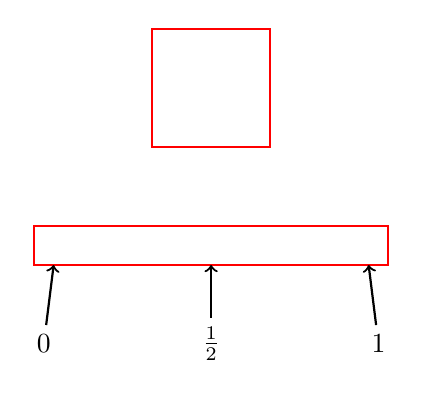
\begin{tikzpicture}[scale=0.5]
    \begin{scope}
        \def\pixels{{10,5,6,2,9},{8,5,2,4,8},{4,8,6,3,1},{2,9,7,10,3},{3,6,6,2,9}}
        \showpixelsvalue{\pixels}{0}{10}
        \draw[red,thick] (2,2) rectangle +(3,3);
    \end{scope}
    \begin{scope}[yshift=-2cm,xshift=-2cm]
        \def\pixels{{2,3,4,5,6,7,8,9,10}} 
        \showpixelsvalue{\pixels}{0}{10}
        \draw[red,thick] (1,1) rectangle +(9,1);
        \draw (1.25,-1) node {$0$} edge[->,thick] (1.5,1);
        \draw (5.5,-1) node {$\frac{1}{2}$} edge[->,thick] (5.5,1);
        \draw (9.75,-1) node {$1$} edge[->,thick] (9.5,1);
    \end{scope}
    \end{tikzpicture}
    \caption{Values in a $3 \times 3$ neighborhood are ordered to define a median (rank 1/2)
    filter. The intensity corresponding to the median value is stored in a new image.}
    \label{fig:median}
\end{figure}

\paragraph{Morphological erosion and dilation} Erosion and dilation are morphological operations on the image. They can be expressed both for binary and grayscale images are the minimum and respectively maximum of the pixels in a neighborhood depicted in red in Figure.~\ref{fig:median}, \textit{i.e.} ranks 0 and 1. In practice, this neighborhood could have various shapes and also have a different weight. Formally, the erosion of a and image $f$ at each pixel $x$ by a structuring element with weights $b$ defined as $(f \oplus b)(x) = \inf_{y} f(x+y) - b(y)$ and the dilation as $(f \ominus b)(x) = \sup_{y} f(y) + b(x-y)$. The result is an image with smaller, and respectively bigger, bright areas enabling to expand and shrink region.

\paragraph{Morphological opening and closing} Opening and closing are also morphological operations resulting of the combination an erosion followed by a dilation, and respectively, the dilation followed by an erosion. Formally, the opening is defined as $f \circ b  = (f \ominus b) \oplus b$ and the closing is defined as $f \bullet  b  = (f \oplus b) \ominus b$.

\paragraph{Rolling ball} Rolling ball~\cite{sternberg1983} is used for correcting shading and non-even background. It works by subtracting a background image estimated by a morphological opening the image using a structuring element which has radially decaying weights (the ball).

\begin{figure}[ht]\centering
    \begin{tikzpicture}[scale=0.8]
        \begin{axis}[
            axis lines=left, 
            xlabel={$x$},
            ylabel={gray levels},
            domain=0:10,
            grid=major,
            samples=200,
            ymin=0.25,
        ]
        \draw [gray,fill,opacity=0.5] (3.4,0.6) ellipse [x radius=1.35, y radius=0.25]; 
        \node (c) at (7,0.6){Rolling ball};
        \addplot[plum1,very thick] {exp(-(x-8)^2 / 100)};
        \addplot[red,very thick] {0.8*exp(-(x-3)^2 / 0.2)+exp(-(x-7)^2 / 0.25)+exp(-(x-8)^2 / 100)};
        \addplot[chameleon1,very thick] {0.055*exp(-(x-3)^2 / 0.4)+0.05*exp(-(x-7)^2 / 0.4)+exp(-(x-8)^2 / 100)};
        \draw[->] (c) -- (5,0.6);
        \end{axis} 
    \end{tikzpicture}
    \caption{Illustration of the rolling ball.}
    \label{fig:algorithm}
\end{figure}

\begin{figure}[ht]\centering
    \begin{tikzpicture}[scale=0.8]
        \begin{axis}[
            axis lines=left, 
            xlabel={$x$},
            ylabel={gray levels},
            domain=0:10,
            grid=major,
            samples=200,
            ymin=0.0,
            ymax=1.2,
        ]
        \addplot[red,very thick,name path=A] {1-(0.7*exp(-(x-2.5)^2 / 0.3)+0.9*exp(-(x-5)^2 / 0.25)+0.6*exp(-(x-8)^2 / 0.5))-0.1*exp(-(x-8)^2 / 80)};
        \addplot+[draw=none, no markers, name path=B] {1}; 
        \addplot[skyblue1,opacity=0.7] fill between[
            of=A and B,
            soft clip={domain=0:3.8}
        ];
        \addplot[plum1,opacity=0.7] fill between[
            of=A and B,
            soft clip={domain=3.8:6.2}
        ];        
        \addplot[chameleon1,opacity=0.7] fill between[
            of=A and B,
            soft clip={domain=6.2:10}
        ];
        
        \end{axis} 
    \end{tikzpicture}
    \caption{Illustration of the watershed algorithms of the digital elevation model (DEM) with 3 flooded depressions. The seeds or sources are the local minima of the DEM.}
    \label{fig:watershed}
\end{figure}



\paragraph{Watershed} The watershed algorithm associate to seed regions pixels in the image in the order of a priority map. It can also be interpreted as flooding a landscape or digital elevation model (DEM) (see Figure~\ref{fig:watershed}). In practice, several algorithms can be considered for implementing a watershed. One of them is called ``priority-flood''~\cite{barnes2014} where starting from seeds, each neighboring pixels (e.g. $3 \times 3$) are added to a queue by order of priority given by a priority map (minimum elevation of the landscape). The queue keeps track of the priority value, the location and the label of the basin. Seeds can be defined as local minima of the landscape function. At each iteration, the highest priority element is popped out of the queue, if not already labeled the pixel if attributed the label of the current basin and its neighbors added to the queue.

\paragraph{Pearson correlation coefficient} The Pearson correlation coefficient (PCC)~\cite{pcc} is a statistical tool used to measure the linear correlation between two signal indicating the potential co-localization of two labelled molecules population. If we have the pair of red and green intensities $(r_i,g_i)$ at each location $i$ in the image, the PCC is defined as 
$$\mathrm{pcc} = \frac{\sum_i(r_i-\bar{r})(g_i-\bar{g})}{\sum_i(r_i-\bar{r})^2 \sum_i(g_i-\bar{g})^2}$$ 
with the means $\bar{r} = n^{-1}\sum_i r_i$ and $\bar{g} = n^{-1}\sum_i g_i$. The value of the PCC ranges from -1 to 1 where a value of 1 indicates a linear correlation.

\paragraph{Table join} To combine measurements from two tables, we can use a ``join''~\cite{join} which will find the  rows base sharing a common reference index. The ``inner join'' operation will include only the matching row in both tables (See Figure~\ref{fig:join}). Manipulating table can replace logical operation on binary masks when combined with object parenting. In the simpler case where table have the same corresponding rows in the same order, tables can be simply collated with each other.

\begin{figure}[ht]\centering
    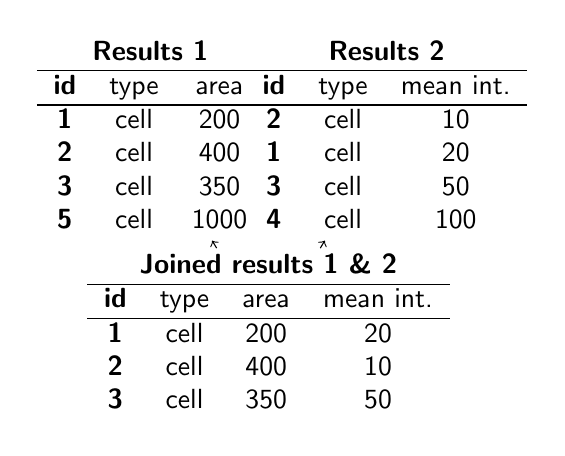
\begin{tikzpicture}
        \node (A) at (0,2.5) {
            \begin{tabular}{>{\bfseries}ccc}
                \multicolumn{3}{c}{\textbf{Results 1}}\\ \hline
                id & type & area \\ \hline
                1  & cell & 200 \\
                2  & cell & 400 \\
                3  & cell & 350  \\
                5 & cell & 1000 
            \end{tabular}
        };
        \node (B) at (3,2.5) {
            \begin{tabular}{>{\bfseries}ccc}
                \multicolumn{3}{c}{\textbf{Results 2}}\\ \hline
                id & type & mean int. \\ \hline
                2  & cell & 10 \\
                1  & cell & 20 \\
                3  & cell & 50 \\
                4  & cell & 100 
            \end{tabular}
        };
        \node (C) at (1.5,0) {
            \begin{tabular}{>{\bfseries}cccc}
                \multicolumn{4}{c}{\textbf{Joined results 1 \& 2}}\\ \hline
                id & type & area & mean int.\\ \hline
                1  & cell & 200 & 20\\
                2  & cell & 400 & 10\\
                3  & cell & 350 & 50
            \end{tabular}
        };
        \draw[->] (A)--(C);
        \draw[->] (B)--(C);
        \end{tikzpicture}
\caption{Inner join of two tables based on the column id.}
\label{fig:join}
\end{figure}



\subsection{Sample preparation and microscopy}

Lots of time can be saved by adjusting sample preparation and imaging to match existing  analysis tools.

\paragraph{Housekeeping labels} If possible, and when aiming at cell level statistics, include extra labels that will help identify cells location during sample preparation. A DNA stains such as DAPI and Hoescht and a plasma membrane marker such as WGA, Invitrogen's CellMask or Biotium's CellBrite can be used for example. 

\paragraph{Cell confluence} Depending on the type of analysis workflow and the cell line, high cell confluence can be counterproductive as cell will tend to grow on top of each other.

\paragraph{Dataset size} When acquiring data, have in mind the scale of the process you want to capture. If only a fraction of the cells are of interest, define multiple position instead of tiling a large field of view at high resolution will reduce the size of the dataset.





 
\newpage
\section{Multi-image splitter}

\subsection{Problem}

Images of Invitrogen's FluoCell prepared slide with BPAE cells stained with MitoTracker Red CMXRos have been acquired on a Nikon ISIM microscope equipped with a multi image splitter. The software then always capture two images. However, only one marker was imaged and we would like to discard the blank image. We want to automatize this task to process several images at once and reduce the size of the dataset. The aim of this example is to illustrate the possibility to modify the original files using a GA3 recipe and potentially loose data.

\paragraph{Dataset} The three files \path{isim_001.nd2} .. \path{isim_003.nd2}  have two channels:
    \begin{enumerate}
        \item Red : Image from the frist camera to keep
        \item Blank : Image to discard
    \end{enumerate}

\paragraph{Concepts} Store results, Batch GA3


\subsection{Step-by-step instructions}
\begin{enumerate} 
    \item Open the image \path{isim_001.nd2} using \menu{File > Open} or a drag and drop.
    \item Open General Analysis 3 (see introduction)
    \item Select the Blank channel and select \menu{Do not Store this Result}. Note that a warning appear now at the bottom of the interface: ``Warning: Execution will remove some existing channels.''
    \item You can run the macro using \menu{Run now}, the image loaded in memory is modified, but the file is not saved.
    \item Save the recipe.
    \item Navigate to \menu{Image > Batch GA3}.
    \item Press the first icon \menu{Add files} and select the recipe and the three \path{isim_001.nd2} .. \path{isim_003.nd2}  files.
    \item Tick \menu{Keep Original} to save the results in a new set of files in a folder  \path{data/recipe_name +++BGM+++_date_time_}
    \item Press \menu{Run}.
    \item The jobs are now also listed under the recipe in the Analysis Explorer.
    \item Open the processed images from the folder \path{data/+++BGM+++_date_time_}
\end{enumerate}
\newpage
\pagebreak
\nsection{Nuclei segmentation}

\begin{description}
    \item[\entry{Task:}] Measure the circularity, mean intensity and area of each nuclei in the image.
    \item[\entry{Data:}] The file “nuclei.tif” has a single channel “Mono”.
    \item[\entry{Topics:}] preprocessing (Rolling Ball, Median), segmentation (Threshold), measurement (Circularity, Mean Obj Intensity, Object Area)
    \item[\entry{Duration:}] 20 min
    \item[\entry{Step by step:}]
\end{description}

\begin{enumerate}
    \item Load the image “nuclei.tif” using “File > Open” or a drag and drop.
    \item Open the General analysis 3 interface using “Image > New GA3 recipe” or a right click on the background, select “Analysis Controls > Analysis Explorer”, select “Create New > General Analysis 3”. 
    \item Correct uneven background. \soln Use \menu{Preprocessing > Rolling Ball} with a radius equal to 26 px and tick \menu{Signal is bright}. \solnend \textcolor{olive}{Radius of the Rolling Ball should be larger than the object of interest.}
    \item Reduce the noise level. \soln For example, using a median filter with \menu{Preprocessing > Median}, set the radius to 2 px. \solnend
    \item Segment the nuclei. \soln Use \menu{Segmentation > Threshold > Threshold}. Set the with an intensity range in [12, 255], Smooth 1x, Clean 1x, FillHoles OFF, Separate 2x, Size[px] 10-max. \solnend
    \item Measure the circularity of the nuclei. \soln Use \menu{Measurement > Object shape > Circularity}. \solnend 
    \item Measure the mean intensity of the nuclei. \soln Use \menu{Measurement > Object intensity > Mean Obj Intensity} by setting the segmented region as the A (Binary) and the input as B (Color). \solnend
    \item Measure the area of the nuclei. \soln Use \menu{Measurement > Object size > Object Area}. \solnend
    \item To group the three records into one single record, press Ctrl and select the three modules the \menu{Circularity}, \menu{MeanObjIntensity} and \menu{ObjectArea} then right click and select “Make Group”.
    \item If needed do the same as in step 8 for RollingBall and Median modules.
\end{enumerate}

\begin{description}
    \item[\entry{Optional:}] scatter plot, find mitosis, etc
\end{description}

\newpage
\section{Synthetic cells}

\subsection{Problem}
In this problem, we make abstraction of the preprocessing steps and focus on the manipulation of binary layers. The image is a sketch representation of three cells with nuclei, cyctosol and some putative vesicles. We want to count the number of vesicle and the area of the nuclei area for each cell.

\begin{center}
\begin{tabular}{rrr}
    Cell ID& Number of endosomes& Nuclei area[px$^2$]\\
    1&8&6562\\
    2&13&7668\\
    3&9&11895\\
\end{tabular}   
\end{center}

\paragraph{Dataset:} The image is \path{synthetic_cells.nd2} with the following channels:
\begin{itemize}\setlength\itemsep{0em}
    \item red: endosomes
    \item green: cytoplasm
    \item blue: nuclei
\end{itemize}

\paragraph{Concepts:} object parenting (ParentID, Child ID, Aggregate Children), data management (GroupRecords, AggegateRows, ModifyColumns, JoinRecords, Aggregate Children), measurement (ObjectArea)

% \begin{description}
%     \item[Task:] For each cell, count the number of red dots and measure the area of the nuclei.
%     \item[Data:] ``synthetic cells.nd2'' with three channels: dots (red), cytoplasm (green) and nuclei (blue). 
%     \item[Topics:] object parenting (ParentID, Child ID, Aggregate Children), data management (GroupRecords, AggegateRows, ModifyColumns, JoinRecords, Aggregate Children), measurement (ObjectArea)
%     \item[Duration:] 30 min
%     \item[Step by step:]
% \end{description}

\subsection{Step-by-step instructions}

\begin{enumerate}
    \item Load the image ``synthetic cells.nd2''.

    \item Create binary masks for all the channels with the names ``endosomes'', ``cells'' and ``nuclei'' \endnote{Use a threshold with value 128-255 for example.}. 

    \item For creating a parent-child hierarchy associating the endosomes to the cells and count the number of endosomes per cell, add the action \menu{Measurement>Object parenting>Aggregate Children} with A (parent): ``cells'' binary and B (child): ``endosomes''. 

    % \begin{description}
    %     \item[Option 1] Associate a parent to each endosome and group the records
    %     \begin{itemize}
    %         \item To associate a cell to each dot,  use \menu{Measurement > Object parenting > Parent ID} linking A (parent) to the ``cytoplasm'' binary and B (child) to the ``dots'' binary.
    %         \item Group the row by adding a module \menu{Data Management > Grouping > Group Records} and use cytoplasmID.    
    %         \item Add the module \menu{Data Management > Grouping >  Aggregate Rows} and set the line ``ObjectId'' to ``Count'' in AggregateRows. 
    %     \end{itemize}

    %     \item[Option 2] Associate a list of child to each cytoplasm and group the records
    %     \begin{itemize}
    %     \item Associate for each cytoplasm, the list of endosomes using \menu{Measurement > Object parenting > Child ID} linking A (parent) to the ``cytoplasm'' binary and B (child) to the ``endosomes'' binary.
    %     \item Group the row by ObjectId using the action \menu{Data Management > Grouping > Group Records} 
    %     \item Add the action \menu{Data Management > Grouping > Aggregate Rows} and set ``dotsID'' to ``Count'' 
    %     \end{itemize}

    %     \item[Option 3] The element ``Aggregate children'' enable to compute parenting and aggregate by parent at once.
    %     \begin{itemize}
    %         \item Drop the module \menu{Measurement>Object parenting>Aggregate Children} on the ``cytoplasm'' binary and link B (child) to the ``endosomes'' binary. 
    %     \end{itemize}
    % \end{description}

    \item Measure the area of each nuclei using \menu{Measurement > Object Size > Object Area}.
    
    \item Add the cell ID to the records of nuclei area using \menu{Measurement > Object parenting > Parent Id} with A (parent) to the ``cell'' and B (child) to the ``nuclei'' binary. 
    
    \item Use \menu{Data Management > Basic > Join Records} to join using ``Object Id'' for tables A and B linking the area measurements and the parenting.
    
    \item Group the row by ``CellId'' using the action \menu{Data Management > Grouping > Group Records} 
    
    \item Add the action \menu{Data Management > Grouping > Aggregate Rows} and set ``Object Area'' to ``Sum'' 
    
    \item Use \menu{Data Management > Basic > Join Records} to join using ``Cell Id'' for tables A and B.
    
    \item Use \menu{Data Management > Basic > Rename Columns} to keep only the necessary columns.

\end{enumerate}

\newpage
\section{Selective cargo tethering}

\subsection{Problem}

In this example, we are interested into quantifying the capture of syntaxin-16 cargos vesicles by the mitochondria when the protein TBC1D23 is relocated to the mitochondria.  Prepared cells were imaged using a Zeiss confocal microscope using a 63x/1.4NA oil immersion lens.

\paragraph{Dataset} We will use the file ``Zeiss1344.lsm'' which have the following channels:
\begin{itemize}\setlength\itemsep{0em}
    \item Ch2-T1 : Golgi maker GM130
    \item ChS2-T2 : cargo protein
    \item ChS1-T3 : mitochondria
    \item Ch1-T4 : nuclei marked with DAPI
\end{itemize}

\paragraph{Concepts} Segmentation with seeded watershed (Threshold, DistanceFunction, Watershed, GrowObjects), colocalization (Pearson Coeff), data management (AppendColumns, Binning, GroupRecords, AppendColumns), display (Barchart).

\paragraph{Credit}  Alison Gillingham from Sean Munro's group at the MRC-LMB

\paragraph{Reference} Jérôme Cattin-Ortolá et al., Cargo selective vesicle tethering: The structural basis for binding of specific cargo proteins by the Golgi tether component TBC1D23. Sci. adv.10,eadl0608(2024). 

DOI:10.1126/sciadv.adl0608

\subsection{Step-by-step instructions}
\begin{enumerate}
    \item Open the image ``Zeiss1344.lsm''.
    \item Segment the cells using a seeded watershed approach by following the three steps below:
    \begin{enumerate}
        \item Create a mask for the cells using the Golgi marker (Ch2-T1) channel. \soln Use \menu{Preprocessing > Convolution > Gaussian Filters} with sigma 2 and \menu{Segmentation>Threshold} with range [1,255]. \solnend
        \item Segment the nuclei. \soln Use \menu{Segmentation>Threshold} with range [30,255], Smooth 5x, Clean OFF, FillHoles OFF, Separate OFF and set the minimal size of the object to \SI{5}{\micro\meter}. \solnend
        \item Separate the touching cells using the nuclei. Drop \menu{Binary processing > Detect > Distance function} onto the Golgi marker (Ch2-T1) binary. Use the \menu{Binary processing> Region growing > Watershed} select the type ``From Bright Regions''. Use \menu{Binary operations > And} linking the result of the watershed (Ch1-T4) and the initial cell mask (Ch2-T1) to restrict the mask to the cells.
    \end{enumerate}
    \item Measure the colocalization of the cargo protein with the Golgi marker (resp the mitochondria). Use \menu{Measurement > Object ratiometry > Pearson Coeff} to measure the colocalization coefficient between the Golgi (Ch2-T1, link to B) and cargo protein (ChS2-T2, link to C) within the segmented region (binary to link to A). Use \menu{Measurement > Object ratiometry > Pearson Coeff} to measure the colocalization coefficient between the mitochondria (ChS1-T3, link to B) and cargo protein (ChS2-T2, link to C) within the segmented region (binary to link to A).
    \item Measure the mean intensity of the mitochondria channel.
    \item Merge the three records table together. \soln Use \menu{Data Management > Basic > AppendColumns}. \solnend
    \item At this point make sure that the workflow doesn’t remove any channel.
    \item Batch process all the other lsm files. Close the GA3 interface and navigate to \menu{Image>Batch GA3}.
    \item Save all the .lsm files as .nd2 files into a different folder while tick the "keep original" option.
    \item Create a figure with the two conditions based on low and high level of mitochondria expression.
\end{enumerate}

% \newpage
% \pagebreak
\nsection{Particle tracking}

\begin{description}
    \item[\entry{Task:}] Track simulated single particle moving in the field of view.
    \item[\entry{Data:}] ``synthetic beads.nd2'' with one channel and 20 time points.
    \item[\entry{Topics:}] Segmentation (Bright Spots), Tracking (Time \& centroid, Track Particles, Accumulate \& group, Speed), Measurement (Mean Obj Intensity), Results (Linechart)
    \item[\entry{Duration:}] 40 min
    \item[\entry{Step by step:}]
\end{description}

\begin{enumerate}
    \item Open the file “synthetic beads.nd2” and create a new General Analysis 3 workflow.
    \item Detect the particles in the image. \soln Use \menu{Segmentation>Spot Detections>Bright Spots} with diameter 0.5 and contrast 2. \solnend
    \item Extract the centroid of each particle. \soln Use the \menu{Tracking>2D Object Position>Time \& Centroid}. \solnend
    \item Measure the mean intensity of each particle. \soln Use \menu{Measurement>Object intensity>Mean Obj Intensity}. \solnend
    \item Merge the two tables to have the centroid and the mean intensity of each particle in one table.  \soln Use \menu{Data Management>Basic>Join Records} using the ObjectId to link the tables A and B. \solnend
    \item Track the particles over time. Use \menu{Tracking > 2D Tracking > Track Particles} with “Time Column” set to "TimeLapseIndex" or "Time"\soln and “Maximum Speed” set to 5 \solnend. Add \menu{Tracking > Tracks > Accumulate \& Group}. \textcolor{olive}{Tracking objects applies to the image while track particle applies to the records; max speed corresponds to max speed of the objects between consecutive frames (however not working in the software at the moment), while max gap size is max allowed skipped frames.}
    \item Measure the speed of each tracked particle. \soln Use \menu{Tracking > Tracking features > Speed} and set “DiffTime” to Time. \solnend
    \item Display the tracks. Use \menu{Results > Linechart}, in the Data tab use “CentroidX” for theh “X Axis” and “CentroidY” for the “Y Axis Left”.
\end{enumerate}

\begin{description}
    \item[\entry{Optional:}] Use the tracking module on the binaries generate by the workflow.
\end{description}

% \newpage
% \section{Infected cells}

\subsection{Problem}




\begin{description}
    \item[Task] Evaluate the number of infected cells by the number of bacteria detected in each of the cells. 
    \item[Data] ``Infected cells.nd2'' with four channels: nuclei marked by DAPI (blue), bac1 (green), bac2 (red), bac3 (cyan).
    \item[Topics] Preprocessing (Gaussian filters), Segmentation (Bright Spots), Binary processing (Grow regions), Data management (Aggregate Children, Append Columns).
    \item[Acknowledgement] Agnes Foeglein
    \item[Duration] 40 min
\end{description}



\subsection{Step-by-step instructions}
\begin{enumerate}
    \item Open the file ``Infected cells.nd2'' and start General Analysis 3
    \item Segment the cells using the DAPI channel. \soln Use \menu{Preprocessing>Gaussian filters} with filter ``Gaussian'' and ``sigma'' 10. Use \menu{Segmentation>Spot Detections>Bright Spot} with diameter 10, contrast 20, symmetry all, Intensity above ``30''. Add \menu{Binary Processing>Region growing>Grow Regions} linking A to the binary and B to the filtered image. \solnend
    \item Segment the bacteria in channels bac1, bac2, bac3. \soln Use \menu{Segmentation > Spot Detections > Bright Spot} with diameter \SI{1}{\micro\meter}, contrast 20, intensity above 150. \solnend
    \item For each cell, count the number of each type of bacteria. \soln Use \menu{Measurement > Object parenting > Aggregate Children} three times with the DAPI binaries as parent and each bac1, bac2, bac3 binaries as children. Merge the 3 tables into one using \menu{Data Management>Basic>Append Columns}. \solnend
\end{enumerate}

% \newpage
% \pagebreak
\nsection{Cell division in dendraster excentricus}

\begin{description}
    \item[\entry{Task:}] Track the cells along the division and count the number of cells over time.
    \item[\entry{Data:}] “cell division.tif” with one channel and 200 time points.
    \item[\entry{Topics:}] preprocessing (Rolling Ball), segmentation (Threshold), object tracking, measurement (Object Count), results (Linechart)
    \item[\entry{Reference:}] 
        George Von Dassow (2011) CIL:15798, Dendraster excentricus. \\
        CIL.Dataset. https://doi.org/doi:10.7295/W9CIL15798
    \item[\entry{Duration:}] 40 min
    \item[\entry{Step by step:}]
\end{description}

\begin{enumerate}
    \item Open the image “cell division.tif” and create a new GA3 workflow.
    \item Segment the nuclei of each cell. \soln Use \menu{Preprocessing>Background>Rolling Ball} with a radius of 10px followed by \menu{Segmentation>Threshold>Threshold} with intensity above 10, Smooth 8x, Clean 1x, FillHoles OFF, Separate 1x and Size[px] above 5px. \solnend
    \item Make sure that the Binaries are stored but that channels are not modified.
    \item Count the number of cell for each time point. Use \menu{Measurement>Whole Field>Object Count} and \menu{Tracking>Tracks>Accumulate \& Group}.
    \textcolor{olive}{I would put these two operations into two separate point; keeping the object count as it is and add the following point for tracking}
    \textcolor{olive}{\item Track the cells over time. Use \menu{Tracking > 2D Tracking > Track Particles} with “Time Column” set to "TimeLapseIndex" or "Time"\soln and “Maximum Speed” set to INF \solnend. Add \menu{Tracking > Tracks > Accumulate \& Group}.}
    \item Graph the number of cells over time. Use \menu{Results>Graphs>Linechart}
    \item Run the recipe on all frames. 
    \item Use the tracking app from the main interface to track all the binaries.
    \textcolor{olive}{Click on tracking options; allow track split; observe from the image stack and estimate how many mitosis happen on average over the time period and determine probability.}
\end{enumerate}


\appendix
\printendnotes

\end{document}
